


\documentclass[30pt,fleqn]{article} 
       
\usepackage[top=3cm,bottom=3cm,left=3.2cm,right=3.2cm,headsep=10pt,letterpaper]{geometry} 

\usepackage{xcolor} 
\definecolor{ocre}{RGB}{52,177,201} 

\usepackage{avant} 
\usepackage{mathptmx} 

\usepackage{microtype} 
\usepackage[utf8]{inputenc}  
\usepackage[T1]{fontenc} 

\usepackage[style=alphabetic,sorting=nyt,sortcites=true,autopunct=true,babel=hyphen,hyperref=true,abbreviate=false,backref=true,backend=biber]{biblatex}


%----------------------------------------------------------------------------------------
%	VARIOUS REQUIRED PACKAGES
%----------------------------------------------------------------------------------------

\usepackage{titlesec} % Allows customization of titles

\usepackage{graphicx} % Required for including pictures
\graphicspath{{Pictures/}} % Specifies the directory where pictures are stored

\usepackage{lipsum} % Inserts dummy text

\usepackage{tikz} % Required for drawing custom shapes

\usepackage[english]{babel} % English language/hyphenation

\usepackage{enumitem} % Customize lists
\setlist{nolistsep} % Reduce spacing between bullet points and numbered lists

\usepackage{booktabs} % Required for nicer horizontal rules in tables

\usepackage{eso-pic} % Required for specifying an image background in the title page

%----------------------------------------------------------------------------------------
%	MAIN TABLE OF CONTENTS
%----------------------------------------------------------------------------------------

\usepackage{titletoc} % Required for manipulating the table of contents

\contentsmargin{0cm} % Removes the default margin
% Chapter text styling
\titlecontents{chapter}[1.25cm] % Indentation
{\addvspace{15pt}\large\sffamily\bfseries} % Spacing and font options for chapters
{\color{ocre!60}\contentslabel[\Large\thecontentslabel]{1.25cm}\color{ocre}} % Chapter number
{}  
{\color{ocre!60}\normalsize\sffamily\bfseries\;\titlerule*[.5pc]{.}\;\thecontentspage} % Page number
% Section text styling
\titlecontents{section}[1.25cm] % Indentation
{\addvspace{5pt}\sffamily\bfseries} % Spacing and font options for sections
{\contentslabel[\thecontentslabel]{1.25cm}} % Section number
{}
{\sffamily\hfill\color{black}\thecontentspage} % Page number
[]
% Subsection text styling
\titlecontents{subsection}[1.25cm] % Indentation
{\addvspace{1pt}\sffamily\small} % Spacing and font options for subsections
{\contentslabel[\thecontentslabel]{1.25cm}} % Subsection number
{}
{\sffamily\;\titlerule*[.5pc]{.}\;\thecontentspage} % Page number
[] 

%----------------------------------------------------------------------------------------
%	MINI TABLE OF CONTENTS IN CHAPTER HEADS
%----------------------------------------------------------------------------------------

% Section text styling
\titlecontents{lsection}[0em] % Indendating
{\footnotesize\sffamily} % Font settings
{}
{}
{}

% Subsection text styling
\titlecontents{lsubsection}[.5em] % Indentation
{\normalfont\footnotesize\sffamily} % Font settings
{}
{}
{}
 
%----------------------------------------------------------------------------------------
%	PAGE HEADERS
%----------------------------------------------------------------------------------------

\usepackage{fancyhdr} % Required for header and footer configuration

\pagestyle{fancy}
\renewcommand{\chaptermark}[1]{\markboth{\sffamily\normalsize\bfseries\chaptername\ \thechapter.\ #1}{}} % Chapter text font settings
\renewcommand{\sectionmark}[1]{\markright{\sffamily\normalsize\thesection\hspace{5pt}#1}{}} % Section text font settings
\fancyhf{} \fancyhead[LE,RO]{\sffamily\normalsize\thepage} % Font setting for the page number in the header
\fancyhead[LO]{\rightmark} % Print the nearest section name on the left side of odd pages
\fancyhead[RE]{\leftmark} % Print the current chapter name on the right side of even pages
\renewcommand{\headrulewidth}{0.5pt} % Width of the rule under the header
\addtolength{\headheight}{2.5pt} % Increase the spacing around the header slightly
\renewcommand{\footrulewidth}{0pt} % Removes the rule in the footer
\fancypagestyle{plain}{\fancyhead{}\renewcommand{\headrulewidth}{0pt}} % Style for when a plain pagestyle is specified

% Removes the header from odd empty pages at the end of chapters
\makeatletter
\renewcommand{\cleardoublepage}{
\clearpage\ifodd\c@page\else
\hbox{}
\vspace*{\fill}
\thispagestyle{empty}
\newpage
\fi}

%----------------------------------------------------------------------------------------
%	THEOREM STYLES
%----------------------------------------------------------------------------------------

\usepackage{amsmath,amsfonts,amssymb,amsthm} % For math equations, theorems, symbols, etc

\newcommand{\intoo}[2]{\mathopen{]}#1\,;#2\mathclose{[}}
\newcommand{\ud}{\mathop{\mathrm{{}d}}\mathopen{}}
\newcommand{\intff}[2]{\mathopen{[}#1\,;#2\mathclose{]}}
\newtheorem{notation}{Notation}[chapter]

%%%%%%%%%%%%%%%%%%%%%%%%%%%%%%%%%%%%%%%%%%%%%%%%%%%%%%%%%%%%%%%%%%%%%%%%%%%
%%%%%%%%%%%%%%%%%%%% dedicated to boxed/framed environements %%%%%%%%%%%%%%
%%%%%%%%%%%%%%%%%%%%%%%%%%%%%%%%%%%%%%%%%%%%%%%%%%%%%%%%%%%%%%%%%%%%%%%%%%%
\newtheoremstyle{ocrenumbox}% % Theorem style name
{0pt}% Space above
{0pt}% Space below
{\normalfont}% % Body font
{}% Indent amount
{\small\bf\sffamily\color{ocre}}% % Theorem head font
{\;}% Punctuation after theorem head
{0.25em}% Space after theorem head
{\small\sffamily\color{ocre}\thmname{#1}\nobreakspace\thmnumber{\@ifnotempty{#1}{}\@upn{#2}}% Theorem text (e.g. Theorem 2.1)
\thmnote{\nobreakspace\the\thm@notefont\sffamily\bfseries\color{black}---\nobreakspace#3.}} % Optional theorem note
\renewcommand{\qedsymbol}{$\blacksquare$}% Optional qed square

\newtheoremstyle{blacknumex}% Theorem style name
{5pt}% Space above
{5pt}% Space below
{\normalfont}% Body font
{} % Indent amount
{\small\bf\sffamily}% Theorem head font
{\;}% Punctuation after theorem head
{0.25em}% Space after theorem head
{\small\sffamily{\tiny\ensuremath{\blacksquare}}\nobreakspace\thmname{#1}\nobreakspace\thmnumber{\@ifnotempty{#1}{}\@upn{#2}}% Theorem text (e.g. Theorem 2.1)
\thmnote{\nobreakspace\the\thm@notefont\sffamily\bfseries---\nobreakspace#3.}}% Optional theorem note

\newtheoremstyle{blacknumbox} % Theorem style name
{0pt}% Space above
{0pt}% Space below
{\normalfont}% Body font
{}% Indent amount
{\small\bf\sffamily}% Theorem head font
{\;}% Punctuation after theorem head
{0.25em}% Space after theorem head
{\small\sffamily\thmname{#1}\nobreakspace\thmnumber{\@ifnotempty{#1}{}\@upn{#2}}% Theorem text (e.g. Theorem 2.1)
\thmnote{\nobreakspace\the\thm@notefont\sffamily\bfseries---\nobreakspace#3.}}% Optional theorem note

%%%%%%%%%%%%%%%%%%%%%%%%%%%%%%%%%%%%%%%%%%%%%%%%%%%%%%%%%%%%%%%%%%%%%%%%%%%
%%%%%%%%%%%%% dedicated to non-boxed/non-framed environements %%%%%%%%%%%%%
%%%%%%%%%%%%%%%%%%%%%%%%%%%%%%%%%%%%%%%%%%%%%%%%%%%%%%%%%%%%%%%%%%%%%%%%%%%
\newtheoremstyle{ocrenum}% % Theorem style name
{5pt}% Space above
{5pt}% Space below
{\normalfont}% % Body font
{}% Indent amount
{\small\bf\sffamily\color{ocre}}% % Theorem head font
{\;}% Punctuation after theorem head
{0.25em}% Space after theorem head
{\small\sffamily\color{ocre}\thmname{#1}\nobreakspace\thmnumber{\@ifnotempty{#1}{}\@upn{#2}}% Theorem text (e.g. Theorem 2.1)
\thmnote{\nobreakspace\the\thm@notefont\sffamily\bfseries\color{black}---\nobreakspace#3.}} % Optional theorem note
\renewcommand{\qedsymbol}{$\blacksquare$}% Optional qed square
\makeatother

% Defines the theorem text style for each type of theorem to one of the three styles above
\newcounter{dummy} 
\numberwithin{dummy}{section}
\theoremstyle{ocrenumbox}
\newtheorem{theoremeT}[dummy]{Theorem}
\newtheorem{problem}{Problem}[chapter]
\newtheorem{exerciseT}{Exercise}[chapter]
\theoremstyle{blacknumex}
\newtheorem{exampleT}{Example}[chapter]
\theoremstyle{blacknumbox}
\newtheorem{vocabulary}{Vocabulary}[chapter]
\newtheorem{definitionT}{Definition}[section]
\newtheorem{corollaryT}[dummy]{Corollary}
\theoremstyle{ocrenum}
\newtheorem{proposition}[dummy]{Proposition}

%----------------------------------------------------------------------------------------
%	DEFINITION OF COLORED BOXES
%----------------------------------------------------------------------------------------

\RequirePackage[framemethod=default]{mdframed} % Required for creating the theorem, definition, exercise and corollary boxes

% Theorem box
\newmdenv[skipabove=7pt,
skipbelow=7pt,
backgroundcolor=black!5,
linecolor=ocre,
innerleftmargin=5pt,
innerrightmargin=5pt,
innertopmargin=5pt,
leftmargin=0cm,
rightmargin=0cm,
innerbottommargin=5pt]{tBox}

% Exercise box	  
\newmdenv[skipabove=7pt,
skipbelow=7pt,
rightline=false,
leftline=true,
topline=false,
bottomline=false,
backgroundcolor=ocre!10,
linecolor=ocre,
innerleftmargin=5pt,
innerrightmargin=5pt,
innertopmargin=5pt,
innerbottommargin=5pt,
leftmargin=0cm,
rightmargin=0cm,
linewidth=4pt]{eBox}	

% Definition box
\newmdenv[skipabove=7pt,
skipbelow=7pt,
rightline=false,
leftline=true,
topline=false,
bottomline=false,
linecolor=ocre,
innerleftmargin=5pt,
innerrightmargin=5pt,
innertopmargin=0pt,
leftmargin=0cm,
rightmargin=0cm,
linewidth=4pt,
innerbottommargin=0pt]{dBox}	

% Corollary box
\newmdenv[skipabove=7pt,
skipbelow=7pt,
rightline=false,
leftline=true,
topline=false,
bottomline=false,
linecolor=gray,
backgroundcolor=black!5,
innerleftmargin=5pt,
innerrightmargin=5pt,
innertopmargin=5pt,
leftmargin=0cm,
rightmargin=0cm,
linewidth=4pt,
innerbottommargin=5pt]{cBox}

% Creates an environment for each type of theorem and assigns it a theorem text style from the "Theorem Styles" section above and a colored box from above
\newenvironment{theorem}{\begin{tBox}\begin{theoremeT}}{\end{theoremeT}\end{tBox}}
\newenvironment{exercise}{\begin{eBox}\begin{exerciseT}}{\hfill{\color{ocre}\tiny\ensuremath{\blacksquare}}\end{exerciseT}\end{eBox}}				  
\newenvironment{definition}{\begin{dBox}\begin{definitionT}}{\end{definitionT}\end{dBox}}	
\newenvironment{example}{\begin{exampleT}}{\hfill{\tiny\ensuremath{\blacksquare}}\end{exampleT}}		
\newenvironment{corollary}{\begin{cBox}\begin{corollaryT}}{\end{corollaryT}\end{cBox}}	

%----------------------------------------------------------------------------------------
%	REMARK ENVIRONMENT
%----------------------------------------------------------------------------------------

\newenvironment{remark}{\par\vspace{10pt}\small % Vertical white space above the remark and smaller font size
\begin{list}{}{
\leftmargin=35pt % Indentation on the left
\rightmargin=25pt}\item\ignorespaces % Indentation on the right
\makebox[-2.5pt]{\begin{tikzpicture}[overlay]
\node[draw=ocre!60,line width=1pt,circle,fill=ocre!25,font=\sffamily\bfseries,inner sep=2pt,outer sep=0pt] at (-15pt,0pt){\textcolor{ocre}{R}};\end{tikzpicture}} % Orange R in a circle
\advance\baselineskip -1pt}{\end{list}\vskip5pt} % Tighter line spacing and white space after remark

%----------------------------------------------------------------------------------------
%	SECTION NUMBERING IN THE MARGIN
%----------------------------------------------------------------------------------------

\makeatletter
\renewcommand{\@seccntformat}[1]{\llap{\textcolor{ocre}{\csname the#1\endcsname}\hspace{1em}}}                    
\renewcommand{\section}{\@startsection{section}{1}{\z@}
{-4ex \@plus -1ex \@minus -.4ex}
{1ex \@plus.2ex }
{\normalfont\large\sffamily\bfseries}}
\renewcommand{\subsection}{\@startsection {subsection}{2}{\z@}
{-3ex \@plus -0.1ex \@minus -.4ex}
{0.5ex \@plus.2ex }
{\normalfont\sffamily\bfseries}}
\renewcommand{\subsubsection}{\@startsection {subsubsection}{3}{\z@}
{-2ex \@plus -0.1ex \@minus -.2ex}
{.2ex \@plus.2ex }
{\normalfont\small\sffamily\bfseries}}                        
\renewcommand\paragraph{\@startsection{paragraph}{4}{\z@}
{-2ex \@plus-.2ex \@minus .2ex}
{.1ex}
{\normalfont\small\sffamily\bfseries}}

%----------------------------------------------------------------------------------------
%	HYPERLINKS IN THE DOCUMENTS
%----------------------------------------------------------------------------------------

% For an unclear reason, the package should be loaded now and not later
\usepackage{hyperref}
\hypersetup{hidelinks,backref=true,pagebackref=true,hyperindex=true,colorlinks=false,breaklinks=true,urlcolor= ocre,bookmarks=true,bookmarksopen=false,pdftitle={Title},pdfauthor={Author}}

%----------------------------------------------------------------------------------------
%	CHAPTER HEADINGS
%----------------------------------------------------------------------------------------

% The set-up below should be (sadly) manually adapted to the overall margin page septup controlled by the geometry package loaded in the main.tex document. It is possible to implement below the dimensions used in the goemetry package (top,bottom,left,right)... TO BE DONE

\newcommand{\thechapterimage}{}
\newcommand{\chapterimage}[1]{\renewcommand{\thechapterimage}{#1}}

% Numbered chapters with mini tableofcontents
\def\thechapter{\arabic{chapter}}
\def\@makechapterhead#1{
\thispagestyle{empty}
{\centering \normalfont\sffamily
\ifnum \c@secnumdepth >\m@ne
\if@mainmatter
\startcontents
\begin{tikzpicture}[remember picture,overlay]
\node at (current page.north west)
{\begin{tikzpicture}[remember picture,overlay]
\node[anchor=north west,inner sep=0pt] at (0,0) {\includegraphics[width=\paperwidth]{\thechapterimage}};
%%%%%%%%%%%%%%%%%%%%%%%%%%%%%%%%%%%%%%%%%%%%%%%%%%%%%%%%%%%%%%%%%%%%%%%%%%%%%%%%%%%%%
% Commenting the 3 lines below removes the small contents box in the chapter heading
%\fill[color=ocre!10!white,opacity=.6] (1cm,0) rectangle (8cm,-7cm);
%\node[anchor=north west] at (1.1cm,.35cm) {\parbox[t][8cm][t]{6.5cm}{\huge\bfseries\flushleft \printcontents{l}{1}{\setcounter{tocdepth}{2}}}};
\draw[anchor=west] (5cm,-9cm) node [rounded corners=20pt,fill=ocre!10!white,text opacity=1,draw=ocre,draw opacity=1,line width=1.5pt,fill opacity=.6,inner sep=12pt]{\huge\sffamily\bfseries\textcolor{black}{\thechapter. #1\strut\makebox[22cm]{}}};
%%%%%%%%%%%%%%%%%%%%%%%%%%%%%%%%%%%%%%%%%%%%%%%%%%%%%%%%%%%%%%%%%%%%%%%%%%%%%%%%%%%%%
\end{tikzpicture}};
\end{tikzpicture}}
\par\vspace*{230\p@}
\fi
\fi}

% Unnumbered chapters without mini tableofcontents (could be added though) 
\def\@makeschapterhead#1{
\thispagestyle{empty}
{\centering \normalfont\sffamily
\ifnum \c@secnumdepth >\m@ne
\if@mainmatter
\begin{tikzpicture}[remember picture,overlay]
\node at (current page.north west)
{\begin{tikzpicture}[remember picture,overlay]
\node[anchor=north west,inner sep=0pt] at (0,0) {\includegraphics[width=\paperwidth]{\thechapterimage}};
\draw[anchor=west] (5cm,-9cm) node [rounded corners=20pt,fill=ocre!10!white,fill opacity=.6,inner sep=12pt,text opacity=1,draw=ocre,draw opacity=1,line width=1.5pt]{\huge\sffamily\bfseries\textcolor{black}{#1\strut\makebox[22cm]{}}};
\end{tikzpicture}};
\end{tikzpicture}}
\par\vspace*{230\p@}
\fi
\fi
}
\makeatother 

\usepackage{listings}
\usepackage{xcolor} % for setting colors

\usepackage{textcomp}


\begin{document}
\date{}
%----------------------------------------------------------------------------------------
%	PORTADA
%----------------------------------------------------------------------------------------

\begingroup
\thispagestyle{empty}
\AddToShipoutPicture*{\put(0,0){
\includegraphics[scale=6.75]{libreta.jpg}}} % FONDO
\centering
\vspace*{5cm}
\par\normalfont\fontsize{35}{35}\sffamily\selectfont
\textbf{Proyecto bases de datos}\\
{\Huge Diseño Papelería}\par % TÍTULO DE TRABAJO
\vspace*{1cm}
{\large Jiménz García María Fernanda }\par
{\large García Cruz Diana Aide}\par % AUTORES
{\large Brandon Silva Barrera}\par
{\large Paul Jaime Félix Flores}\par

\endgroup

%----------------------------------------------------------------------------------------
%	DATOS
%----------------------------------------------------------------------------------------


~\vfill
\thispagestyle{empty}

\noindent \textsc{UNIVERSIDAD NACIONAL AUTÓNOMA DE MÉXICO}\\

\noindent \textsc{Bases de Datos}\\ % URL

\noindent \textit{Fecha de entrega: 27 de mayo de 2020} 

%------------------------------------------------------------------------------
%	CONTENIDO
%------------------------------------------------------------------------------
\newpage
\pagestyle{empty} 

\tableofcontents % contenido

\pagestyle{fancy} 

%-----------------------------------------------------------------------------
%	INTRODUCCION
%-----------------------------------------------------------------------------

\newpage

%\chapterimage{abstract.png}  

% Definimos el título
\title{Proyecto base de datos:Implementación de papelería}

\maketitle 

\section{Introducción}\index{Introducción}
\vspace{5mm} %5mm vertical space
El presente documento muestra el desarrollo del análisis, diseño y propuesta de implementación de una base de datos de para el almacenamiento de información de una papelería, de esta manera ayudará a la empresa a organizar, controlar y administrar los productos y las ventas, mejorando la interacción con los clientes. 


\subsection{Objetivo}
\vspace{5mm} %5mm vertical space
Cada vez más empresas optan por implementar sistemas de gestión de ventas utilizando las tecnologías de información con el objetivo de incrementar los clientes y potenciales clientes, además de las ventas.

Por lo tanto, para el caso de una empresa de ventas de productos de papelería, se desarrolla un sistema de tienda virtual para la gestión de ventas que permita a los clientes registrarse, seleccionar los productos, comprarlos y pagarlos.

Implementar un sistema de tienda virtual genera diversos beneficios como: Manejar un registro de clientes, manejar un registro de ventas, permitir emitir reportes de ventas, clientes y productos actualizados que ayudan a la empresa a tomar mejores decisiones a corto y a largo plazo. 


\begin{figure}[h]
    \centering
    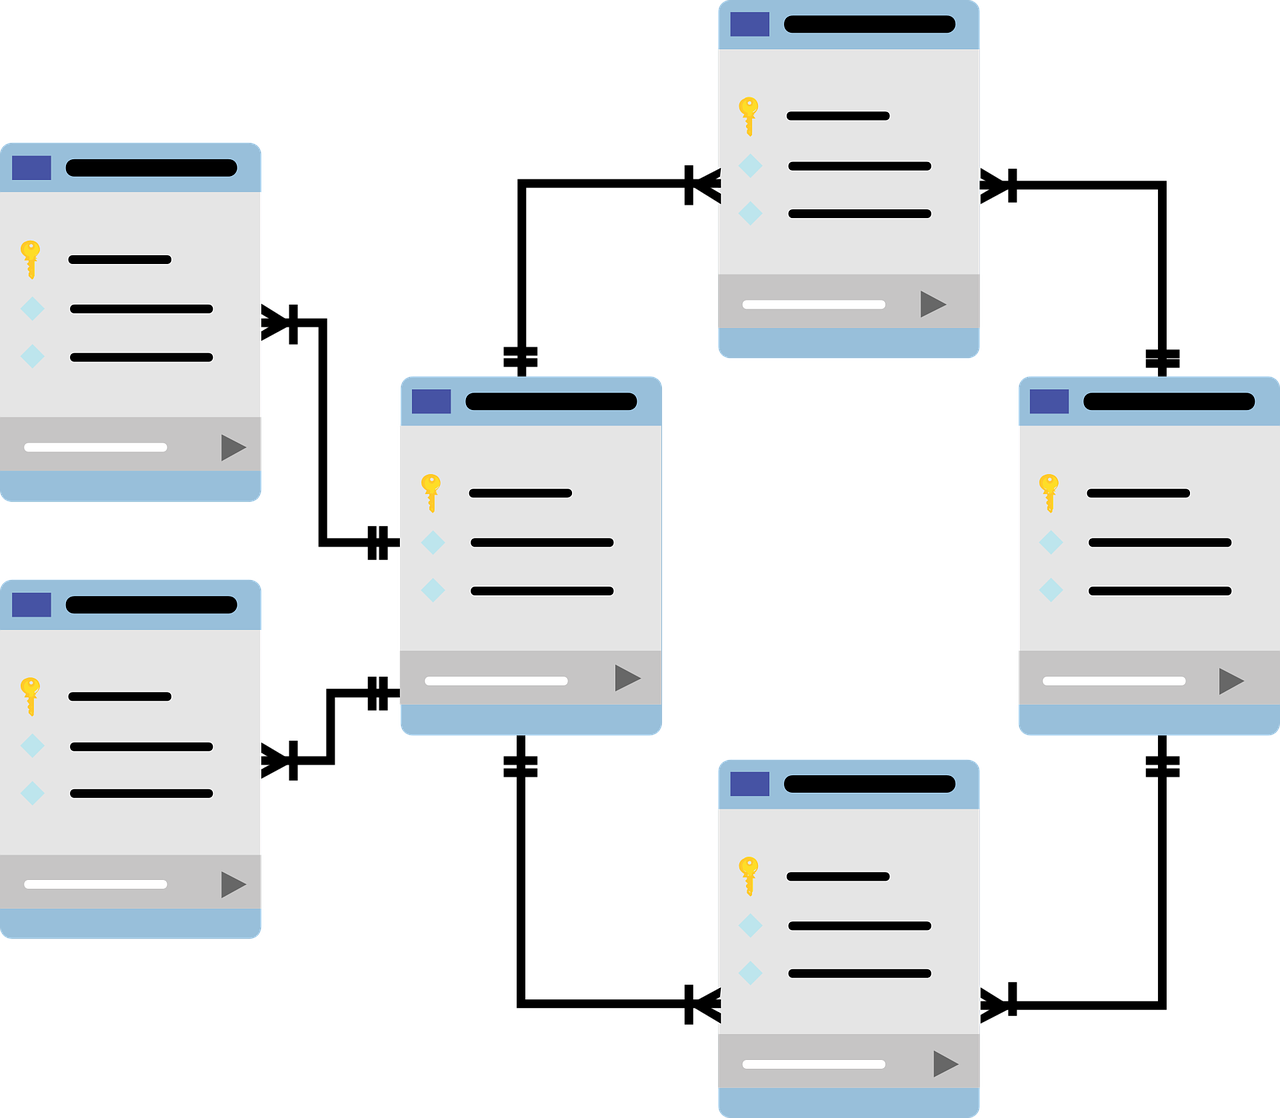
\includegraphics[width=0.57\textwidth]{base.png}\hspace{1cm}
    \caption{Diseño de base de datos}
    \label{fig:Database}
\end{figure}
\vspace{10mm} %5mm vertical space
 
\subsection{Descripción del análisis del problema}
\vspace{5mm} %5mm vertical space
El proyecto requirió realizar un sistema informático para la administración de una papelería, de manera que los datos cambien en tiempo real y se mantengan consistentes siguiendo ciertas reglas de negocio. Para hacer lo anterior posible se siguieron las siguientes condiciones.
\vspace{5mm} %5mm vertical space

\begin{itemize}
\item El sistema maneja el inventariado de los productos almacenando sus características	principales y su proveedor, a la vez que mantiene sus existencias(stock).
\item Tiene un registro de los proveedores y su información.
\item Almacena información de los clientes.
\item Hace posible un proceso de ventas, de manera que en la venta registre el cliente, los  productos que la conforman y un identificador único. Los productos vendidos se deben retirar del inventario. Además se debe calcular el monto total y el monto por cada artículo.  
\end{itemize}


%-----------------------------------------------------------------------------
% PLAN DE TRABAJO
%-----------------------------------------------------------------------------
\vspace{5mm} %5mm vertical space
\section{Plan de trabajo}\index{Plan de trabajo}

Primero se hizo un análisis de los componentes con los que ya contaban dos equipos que conformaron el actual. 

Se decidió adaptar los componentes de ambos con la finalidad de unir sus respectivos trabajos.
Así, dos personas se encargaron del diseño de la base de datos y dos de la interfaz gráfica. 

\vspace{5mm} %5mm vertical space

\begin{itemize}
\item \textit{García Cruz Diana Aide} 

\vspace{5mm} %5mm vertical space

\textbf{Diseño e implementación de la base de datos:}

Diseño de modelos entidad-relación y modelo relacional.
Normalización de base de datos.
Implementación en lenguaje SQL de base de datos y tablas.
Participación en agregado de información.
Implementación de consultas y funciones.

\vspace{5mm} %5mm vertical space

\item \textit{Jiménez García María Fernanda} 

\vspace{5mm} %5mm vertical space

\textbf{Diseño e implementación de la base de datos:}

Diseño de modelos entidad-relación y modelo relacional.
Normalización de base de datos.
Implementación en lenguaje SQL de base de datos y tablas.
Participación en agregado de información.
Implementación de consultas y funciones.

\textbf{Documentación:}
Redactada en latex.

\vspace{5mm} %5mm vertical space

\item \textit{Brandon Silva Barrera} 

\vspace{5mm} %5mm vertical space

Participó en la documentación y unión de los elementos de ambos equipos que se decidió reutilizar, además que actuó como elemento de apoyo en otras áreas. 

\vspace{5mm} %5mm vertical space

\item \textit{Paul Jaime Félix Flores} 
\vspace{5mm} %5mm vertical space

Implementación de interfaz gráfica en java.
Adaptación de la interfaz de usuario en java a la base de datos.


\end{itemize}




%-----------------------------------------------------------------------------
%	DISEÑO
%-----------------------------------------------------------------------------

\newpage
\section{Diseño}\index{Diseño}
\vspace{5mm} %5mm vertical space

\textbf{Enunciado:}
\vspace{6mm} %10mm vertical space
Una cadena de papelerı́as busca innovar la manera en que almacena su información, y los contratan para que desarrollen los sistemas informáticos para satisfacer los siguientes requerimientos:

Se desea tener almacenados datos como la razón social,domicilio, nombre y teléfonos de los proveedores, razón social, nombre, domicilio y al menos un email de los clientes. Es necesario tener un inventario de los productos que se venden, en el que debe guardarse el código de barras, precio al que fue comprado el producto, fecha de compra y cantidad de ejemplares en la bodega (stock).

Se desea guardar la marca, descripción y precio de los regalos, artı́culos de
papelerı́a, impresiones y recargas, siempre y cuando se tenga su correspondiente registro en el inventario. Debe también guardarse el número de venta, fecha de venta y la cantidad total a pagar de la venta, ası́ como la cantidad de cada artı́culo y precio total a pagar por artı́culo.
Además, se requiere que:

-Al recibir el código de barras de un producto, regrese la utilidad.

-Cada que haya la venta de un artı́culo, deberá decrementarse el stock por
la cantidad vendida de ese artı́culo.

-Si el valor llega a cero, abortar la transacción. Si hay menos de 3, emitir un mensaje.

-Dada una fecha, o una fecha de inicio y fecha de fin, regresar la cantidad
total que se vendió en esa fecha/periodo.1

-Permitir obtener el nombre de aquellos productos de los cuales hay menos
de 3 en stock.

-De manera automática se genere una vista que contenga información necesaria para asemejarse a una factura de una compra.

-Crear al menos, un ı́ndice, del tipo que se prefiera y donde se prefiera.
Justificar el porqué de la elección en ambos aspectos.


-El número de venta debe tener un formato similar a ”VENT-001”, prefijo
VENT, seguido de un guión y un número secuencial.

-Donde este presente el atributo domicilio, está compuesto por estado,
código postal, colonia, calle y número.

-El diseño debe satisfacer todos los principios de diseño, los requerimientos
anteriores y un buen manejo de información.

\begin{figure}[h]
    \centering
    
\includegraphics[width=0.35\textwidth]{req.png}
    \caption{Requerimientos}
    \label{fig:Requerimientos}
\end{figure}

\subsection{Análisis general}

\vspace{5mm} %5mm vertical space

Se realizará un sistema de ventas para una papelería, para poder tener un registro de los productos que se almacenan, así como las ventas que se realicen.

El objetivo de la base de datos es dar seguimiento a datos tales como clientes, empleados,proveedores, inventario y productos con su respectiva categoría. Sin embargo, cabe mencionar que la conexión entre todos ellos, la encontramos centrada las ventas de los productos.Por lo que también se consideró como una entidad. Los atributos y relaciones, se especificarán en el siguiente apartado.



%-----------------------------------------------------------------------------
%	MER
%-----------------------------------------------------------------------------

\subsection{Modelo Entidad-Relación.}

\vspace{5mm} %5mm vertical space

Los elementos del modelo entidad – relación  a identificar son: entidades, atributos, identificadores y relaciones.

\vspace{5mm} %5mm vertical space

\begin{itemize}
\vspace{5mm} %5mm vertical space
\item\textbf{Entidad: Objeto exclusivo único en el mundo real que se está controlando.Se se quiere dar seguimiento.}

\vspace{5mm} %5mm vertical space

Entidades identificadas:
\begin{itemize}

\vspace{5mm} %5mm vertical space
\item PROVEEDOR:Se desea almacenar información de aquel que provee productos. 

\vspace{5mm} %5mm vertical space


\item PRODUCTO:Se desea almacenar información del producto para venderlo al cliente y tener un registro en el inventario.

\vspace{5mm} %5mm vertical space

\item CATEGORÍA:Se desea dividir en distintas categorías los respectivos productos

\vspace{5mm} %5mm vertical space

\item INVENTARIO: Se desea almacenar información de los productos que nos permitan relacionarlos con las ventas, dado que tenemos que un precio de compra al proveedor y un precio de venta al cliente, esto con la finalidad de obtener la utilidad.

\vspace{5mm} %5mm vertical space

\item VENTA: Se desea almacenar información de las ventas, de manera que se permita gestionar la salida de los productos y ofrecer un servicio óptimo al cliente.

\vspace{5mm} %5mm vertical space

\item CLIENTE:Se desea almacenar información de aquella persona que utilice los servicios de la papelería, especialmente de la que lo hace regularmente.

\vspace{5mm} %5mm vertical space
\end{itemize}
\vspace{10mm} %5mm vertical space

\begin{figure}[h]
    \centering
    
\includegraphics[width=0.75\textwidth]{entidad.jpg}
    \caption{Entidad}
    \label{fig:Entidad}
\end{figure}

\vspace{10mm} %5mm vertical space
\vspace{10mm} %5mm vertical space
\item\textbf{Atributos: Característica o rasgo de un tipo de entidad que describe la entidad.}
\vspace{10mm} %5mm vertical space

\begin{itemize}
\item PROVEEDOR:id, nombre, razón social, domicilio y teléfono
\vspace{10mm} %5mm vertical space
\item PRODUCTO:id, marca, descripción, precio.
\vspace{10mm} %5mm vertical space
\item CATEGORÍA:id, descripción.
\vspace{10mm} %5mm vertical space
\item INVENTARIO: codigo de barras, precio de compra, fecha de compra, stock, precio de venta.
\vspace{10mm} %5mm vertical space
\item VENTA: id, fecha, total
\vspace{10mm} %5mm vertical space
\item CLIENTE:id, nombre, razón social, domicilio e email
\end{itemize}
\vspace{10mm} %5mm vertical space
\vspace{10mm} %5mm vertical space

\item \textbf{Identificadores: son atributos que identifican las instancias de una entidad. }
\vspace{10mm} %5mm vertical space

\begin{itemize}

\item PROVEEDOR:identificado por idProv
\vspace{10mm} %5mm vertical space
\item PRODUCTO:identificado por idProd
\vspace{10mm} %5mm vertical space
\item CATEGORÍA:identificado por idCategoria
\vspace{10mm} %5mm vertical space
\item INVENTARIO: identificado por codBarras
\vspace{10mm} %5mm vertical space
\item VENTA:identificado por  idVenta
\vspace{10mm} %5mm vertical space
\item CLIENTE:identificado por idCliente
\vspace{10mm} %5mm vertical space

\end{itemize}


\vspace{10mm} %5mm vertical space
\vspace{10mm} %5mm vertical space
\item \textbf{Relaciones: las entidades se pueden asociar con otras mediante relaciones. Existen tres tipos de relaciones: 1..1 (uno a uno), 1..m (uno a muchos) y m..m (muchos a muchos). }

\vspace{10mm} %5mm vertical space

El sistema guardara informacion de las categorias que se vendan por ejemplo: lapiz, libreta, borrador, etc, de las categorias se almanece un idCategoria y su descrpición. 

\vspace{10mm} %5mm vertical space
Tambien se almacenara informacion de los proveedores que surtan la papeleria, en este caso seria del contacto(idProveedor, nombre, telefono).

\vspace{10mm} %5mm vertical space
De los productos se deseara almacenar (el id del producto, marca, precio,descripcion, stock).
1 categoria aparece en varios productos y 1 producto solo tiene 1 categoria. 1 proveedor surte varios productos y 1 producto es surtido por un solo proveedor.

\vspace{10mm} %5mm vertical space
En el inventario se almacenaran los productos con su respectivo id, pero así mismo, se le asignará un código de barras,que se asociará con las ventas. Tenemos un precio de compra al proveedor, pero al requerir una utilidad por producto, el precio de venta al cliente, sería más elevado. También al tener un registro de los productos almacenados, en el atributo stock tendremos un control sobre los que aún se encuentran en bodega, y así, cuando los productos estén por terminarse, se comprarán más al proveedor.

\vspace{10mm} %5mm vertical space

La papeleria cuenta con un sistema de ventas.
Se debera llevar tambien un registro de las ventas que se realicen en la papeleria , por cada venta se almacenara un idVenta, fecha y el total de la venta. Una venta tiene muchos productos y 1 producto puede estar en varias ventas.

\vspace{10mm} %5mm vertical space

De los clientes que hagan una venta se tendrá un idCliente, nombre, apellido paterno, apellido materno, direccion e email(pueden ser varios, al menos uno).

Un cliente realiza muchas ventas, 1 venta solo es realizada por 1 cliente.


\vspace{10mm} %5mm vertical space

Tambien se cuenta con usuarios(empleados) que seran los que se encargaran de realizar ventas y crear apartados, de ellos se almacena un idEmpleado, nombreUsuario y contraseña. 1 empleado puede realizar muchas ventas, pero una venta es realizada por un solo empleado, tambien un empleado crea varios apartados pero 1 apartado es creado por un solo usuario.


\end{itemize}

\vspace{50mm} %5mm vertical space
\item\textbf{Modelo Entidad Relación final}


\begin{figure}[h]
    \centering
    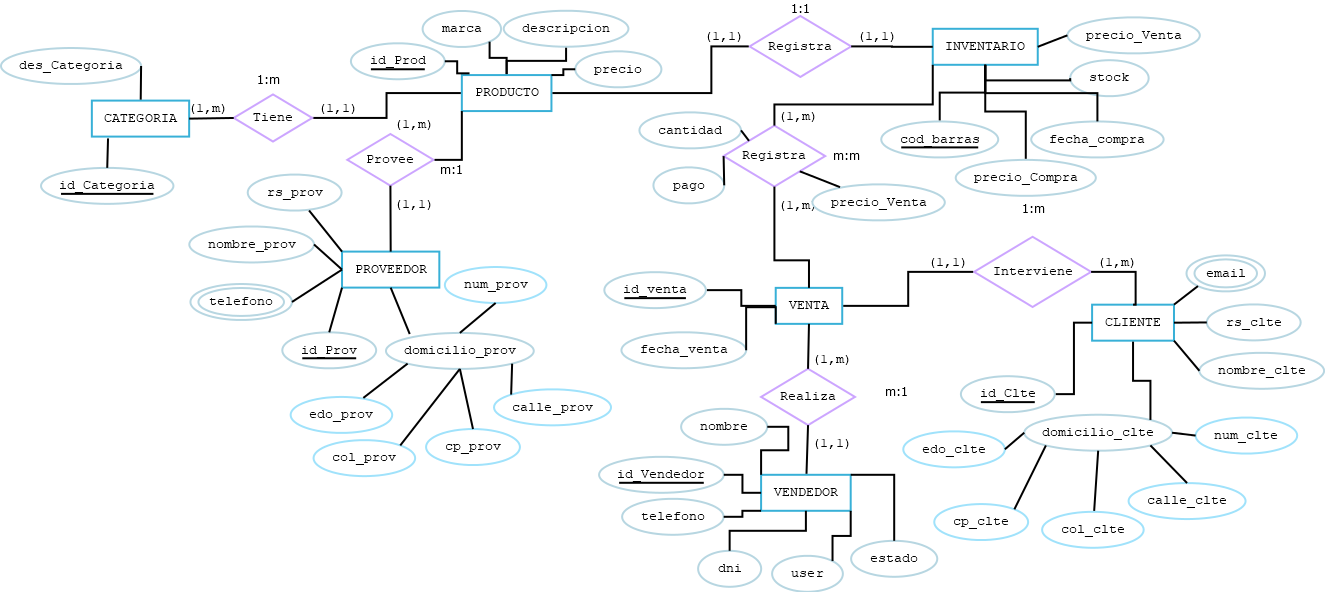
\includegraphics[width=0.95\textwidth]{ER.png}
    \caption{Modelo Entidad Relación}
    \label{fig:Modelo Entidad Relació}
\end{figure}

\vspace{10mm} %5mm vertical space

%-------------------------------------------------------------------------
\subsection{Modelo Relacional}

\vspace{5mm} %5mm vertical space

Modelo de organización y gestión de bases de datos consistente en el almacenamiento de datos en tablas compuestas por filas, o tuplas, y columnas o campos.

\vspace{5mm} %5mm vertical space

\begin{itemize}
\vspace{5mm} %5mm vertical space
\item\textbf{Mapeo Entidades:}
\end{itemize}

\vspace{10mm} %5mm vertical space
 PROVEEDOR {id_Prov (Pk), rs_Prov, nom_Prov, apPat_Prov,apMat_Prov, cp_Pov, col_Prov, calle_Prov num_Prov}
 
 \vspace{10mm} %5mm vertical space
 
TELEFONO-PROVEEDOR {id_Prov(PK, FK), telefono(PK) } 

\vspace{10mm} %5mm vertical space

CLIENTE{ id_Cliente, rs_Cliente, nom_Cliente, edo_Cliente, cp_Cliente, col_Cliente, calle_Cliente, num_Cliente}

\vspace{10mm} %5mm vertical space

EMAIL-CLIENTE {id_Cliente(FK,PK), email} 
CATEGORIA {id_Categoria (PK), nom_Categoria}

\vspace{10mm} %5mm vertical space

PRODUCTO {id_Prod (PK), id_Prov(FK), id_Categoria (FK), marca, descripcion, precio}

\vspace{10mm} %5mm vertical space

INVENTARIO { cod_Barras (PK), id_Prod (FK), precio_Compra, precio_Venta fecha_Compra, stock} 

\vspace{10mm} %5mm vertical space

VENTA {id_Venta(PK), id_Cliente (FK), fecha_Venta, cant_art, precio_art}

\vspace{10mm} %5mm vertical space

REGISTRAR {[cod_Barras (FK), id_Venta (FK)] (PK), precio_Venta, cantidad, pago, total}

\vspace{10mm} %5mm vertical space

VENDEDOR {id_Vendedor(PK), nombre, DNI, user, estado}

 \vspace{10mm} %5mm vertical space
 
TELEFONO-VENDEDOR {id_Vend(PK, FK), telefono(PK) } 

\vspace{10mm} %5mm vertical space


\vspace{20mm} %5mm vertical space
\item\textbf{Modelo Relacional}

\vspace{10mm} %5mm vertical space

\begin{figure}[h]
    \centering
    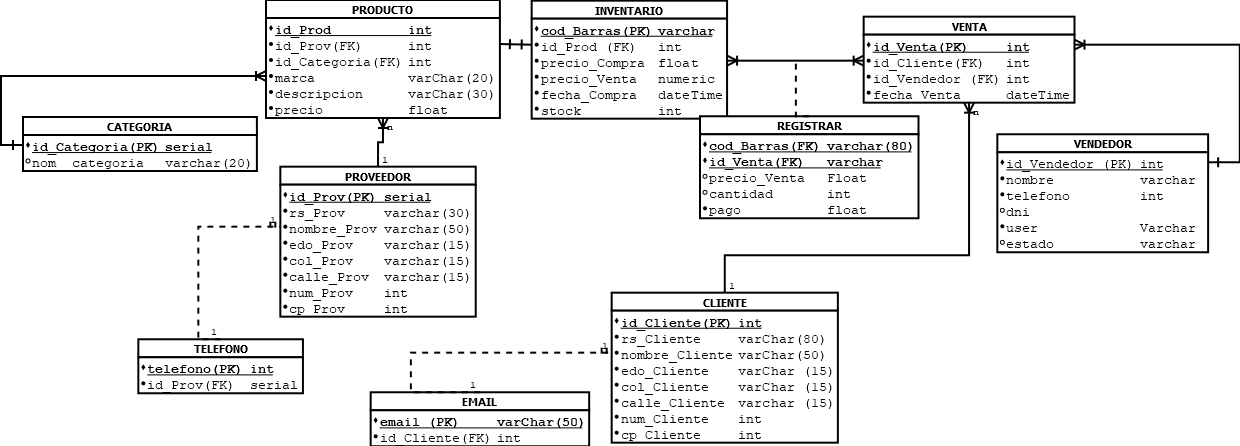
\includegraphics[width=0.95\textwidth]{MR.png}
    \caption{Modelo Relacional}
    \label{fig:Modelo Relacional}
\end{figure}

\subsection{Normalización}
\vspace{10mm} %5mm vertical space

CUMPLEN 1FN
\vspace{10mm} %5mm vertical space

 PROVEEDOR {id_Prov (Pk), rs_Prov, nom_Prov, apPat_Prov,apMat_Prov, cp_Pov, col_Prov, calle_Prov num_Prov}
 
 \vspace{10mm} %5mm vertical space
 
TELEFONO-PROVEEDOR {id_Prov(PK, FK), telefono(PK) } 

\vspace{10mm} %5mm vertical space

CLIENTE{ id_Cliente, rs_Cliente, nom_Cliente, edo_Cliente, cp_Cliente, col_Cliente, calle_Cliente, num_Cliente}

\vspace{10mm} %5mm vertical space

EMAIL-CLIENTE {id_Cliente(FK,PK), email} 
CATEGORIA {id_Categoria (PK), nom_Categoria}

\vspace{10mm} %5mm vertical space

PRODUCTO {id_Prod (PK), id_Prov(FK), id_Categoria (FK), marca, descripcion, precio}

\vspace{10mm} %5mm vertical space

INVENTARIO { cod_Barras (PK), id_Prod (FK), precio_Compra, precio_Venta fecha_Compra, stock} 

\vspace{10mm} %5mm vertical space

VENTA {id_Venta(PK), id_Cliente (FK), fecha_Venta, cant_art, precio_art}

\vspace{10mm} %5mm vertical space

REGISTRAR {[cod_Barras (FK), id_Venta (FK)] (PK), precio_Venta, cantidad, pago, total}

\vspace{10mm} %5mm vertical space

VENDEDOR {id_Vendedor(PK), nombre, DNI, user, estado}

 \vspace{10mm} %5mm vertical space
 
TELEFONO-VENDEDOR {id_Vend(PK, FK), telefono(PK) } 

 \vspace{10mm} %5mm vertical space 
 
 \vspace{10mm} %5mm vertical space
CUMPLEN 2FN
\vspace{10mm} %5mm vertical space

 PROVEEDOR {id_Prov (Pk), rs_Prov, nom_Prov, apPat_Prov,apMat_Prov, cp_Pov, col_Prov, calle_Prov num_Prov}
 
 \vspace{10mm} %5mm vertical space
 
TELEFONO-PROVEEDOR {id_Prov(PK, FK), telefono(PK) } 

\vspace{10mm} %5mm vertical space

CLIENTE{ id_Cliente, rs_Cliente, nom_Cliente, edo_Cliente, cp_Cliente, col_Cliente, calle_Cliente, num_Cliente}

\vspace{10mm} %5mm vertical space

EMAIL-CLIENTE {id_Cliente(FK,PK), email} 
CATEGORIA {id_Categoria (PK), nom_Categoria}

\vspace{10mm} %5mm vertical space

PRODUCTO {id_Prod (PK), id_Prov(FK), id_Categoria (FK), marca, descripcion, precio}

\vspace{10mm} %5mm vertical space

INVENTARIO { cod_Barras (PK), id_Prod (FK), precio_Compra, precio_Venta fecha_Compra, stock} 

\vspace{10mm} %5mm vertical space

VENTA {id_Venta(PK), id_Cliente (FK), fecha_Venta, cant_art, precio_art}

\vspace{10mm} %5mm vertical space

REGISTRAR {[cod_Barras (FK), id_Venta (FK)] (PK), precio_Venta, cantidad, pago, total}

\vspace{10mm} %5mm vertical space

VENDEDOR {id_Vendedor(PK), nombre, DNI, user, estado}

 \vspace{10mm} %5mm vertical space
 
TELEFONO-VENDEDOR {id_Vend(PK, FK), telefono(PK) } 


 \vspace{10mm} %5mm vertical space

\vspace{10mm} %5mm vertical space
No cumple 2FN
\vspace{10mm} %5mm vertical space

REGISTRAR {[cod_Barras (FK), id_Venta (FK)] (PK), precio_Venta, cantidad, pago, total}

\vspace{10mm} %5mm vertical space

Normalizando

 \vspace{10mm} %5mm vertical space

REGISTRAR {[cod_Barras (FK), id_Venta (FK)] (PK), precio_Venta, cantidad, pago}


\vspace{10mm} %5mm vertical space

Agregamos atributos para facturación automática

\vspace{10mm} %5mm vertical space

REGISTRAR-PAGO{id_Venta (PK),subtotal, IVA, total}



%----------------------------------------------------------------------------------------
%	IMPLEMENTACION
%-----------------------------------------------------------------------------
-------------------

\newpage
\section{Implementación}\index{Implementación}

\subsection{Base de datos}\index{Base de datos}

\begin{figure}[h]
    \centering
    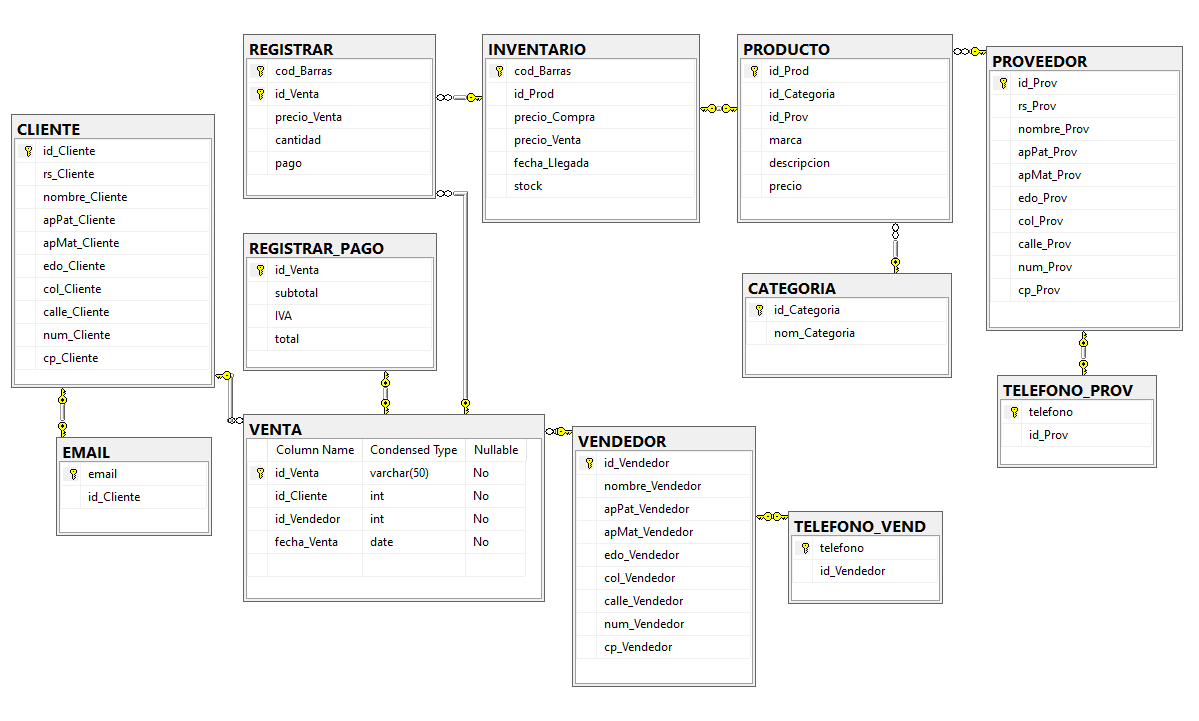
\includegraphics[width=0.95\textwidth]{Papeleria.png}
    \caption{Modelo Relacional}
    \label{fig:Modelo Relacional}
\end{figure}
\vspace{5mm} %5mm vertical space


\newpage
\subsection{Creación de tablas}\index{Creación de tablas}


%----------------------------------------------------------------------------------------------------------------------------------------------------
\definecolor{AzulClaro}{rgb}{0.2,0.5,0.7}
% set the default code style
\lstset{
    frame=tb, % draw a frame at the top and bottom of the code block
    tabsize=4, % tab space width
    showstringspaces=false, % don't mark spaces in strings
    numbers=left, % display line numbers on the left
    commentstyle=\color{AzulClaro}, % comment color
    keywordstyle=\color{blue}, % keyword color
    stringstyle=\color{red} % string color
}

%---------------------------------------------------------------------------------------------------------------------------------------------------------

\begin{lstlisting}[language=sql, caption={DDL.Estructura de base de datos Papelería. }]

/*ALMACENAMIENTO DE DATOS DE PERSONAS (PROVEEDORES,CLIENTES, VENDEDORES)*/

CREATE TABLE PROVEEDOR(
    id_Prov serial,
    rs_Prov varchar (80) not null, 
    nombre_Prov varchar (30) not null,
	apPat_Prov varchar (30) not null,
	apMat_Prov varchar (30) null,
	edo_Prov varchar (30) not null,
	col_Prov varchar(30) not null,
	calle_Prov varchar(30) not null,
	num_Prov varchar(30) not null,
	cp_Prov int not null,
	CONSTRAINT "PK_PROVEEDOR" PRIMARY KEY (id_Prov)
);
/*Se registra el teléfono de proveedores en una nueva tabla, 
con la finalidad de evitar campos multivaluados, dado que se
puede almacenar más de un campo*/

CREATE TABLE TELEFONO_PROV(
	telefono int not null,
	id_Prov serial,
	UNIQUE (id_prov),
	CONSTRAINT "PK_TELEFONO_PROV" PRIMARY KEY (telefono),
	CONSTRAINT "FK_TELEFONO_PROVEEDOR" FOREIGN KEY (id_Prov)
	REFERENCES PROVEEDOR(id_Prov)
);

--------------------------------------------------------------------------------
CREATE TABLE CLIENTE(
	id_Cliente serial,
	rs_Cliente varchar (80) not null,
    nombre_Cliente varchar (30) not null,
	apPat_Cliente varchar (30) not null,
	apMat_Cliente varchar (30) null,
	edo_Cliente varchar (30) not null,
	col_Cliente varchar(30) not null,
	calle_Cliente varchar (30) not null,
	num_Cliente varchar(30) not null,
	cp_Cliente int not null,
	CONSTRAINT "PK_CLIENTE" PRIMARY KEY (id_cliente)
);

/*Se registra el email de clientes en una nueva tabla, 
con la finalidad de evitar campos multivaluados (Se almacena al menos
uno, con la restricción de no aceptar registros nulos, pero pueden
ser más.*/
CREATE TABLE EMAIL(
	email varchar(50) not null, 
	id_Cliente serial,
	UNIQUE (id_Cliente),
	CONSTRAINT "PK_EMAIL" PRIMARY KEY (email),
	CONSTRAINT "FK_EMAIL_CLIENTE" FOREIGN KEY (id_Cliente)
	REFERENCES CLIENTE(id_Cliente)
);

--------------------------------------------------------------------------------

CREATE TABLE VENDEDOR(
	id_Vendedor serial,
    nombre_Vendedor varchar (30) not null,
	apPat_Vendedor varchar (30) not null,
	apMat_Vendedor varchar (30) null,
	edo_Vendedor varchar (30) not null,
	col_Vendedor varchar(30) not null,
	calle_Vendedor varchar (30) not null,
	num_Vendedor varchar(30) not null,
	cp_Vendedor int not null,
	CONSTRAINT "PK_VENDEDOR" PRIMARY KEY (id_Vendedor)
);

/*Se registra el teléfono de proveedores en una nueva tabla, 
con la finalidad de evitar campos multivaluados, dado que se
puede almacenar más de un campo*/


CREATE TABLE TELEFONO_VEND(
	telefono int not null,
	id_Vendedor serial,
	UNIQUE (id_Vendedor ),
	CONSTRAINT "PK_TELEFONO_VEN" PRIMARY KEY (telefono),
	CONSTRAINT "FK_TELEFONO_VENDEDOR" FOREIGN KEY (id_Vendedor )
	REFERENCES VENDEDOR(id_Vendedor)
);

--------------------------------------------------------------------------------

/*ALMACENAMIENTO DE INFORMACIÓN RELACIONADA A LOS PRODUCCTOS*/


--Creacion de indice
--CREATE INDEX Indice_Categoria on CATEGORIA(id_Categoria);

CREATE TABLE CATEGORIA (
	id_Categoria serial,
	nom_Categoria varchar (30),
	CONSTRAINT "PK_CATEGORIA" PRIMARY KEY (id_categoria)
);

CREATE TABLE PRODUCTO(
	id_Prod serial,
	id_Categoria int not null,--serial,
	id_Prov int not null,--serial,
	marca varChar (60),
	descripcion varchar (30),
	precio numeric not null,
	CONSTRAINT "PK_PRODUCTO" PRIMARY KEY (id_Prod),
    CONSTRAINT "FK_PRODUCTO_CATEGORIA" FOREIGN KEY (id_Categoria)
	REFERENCES CATEGORIA(id_Categoria),
	CONSTRAINT "CK_PRECIO_PRODUCTO" CHECK (precio>0),
	CONSTRAINT "FK_PRODUCTO_PROVEEDOR" FOREIGN KEY (id_Prov)
	REFERENCES PROVEEDOR(id_Prov)
);

/*Almacena información de los productos, relacionada a la compra al proveedor.

Así mismo se asigna un codigo de barras por producto y el precio de venta al cliente.

Por otra parte tenemos el atributo stock que nos permite tener un control sobre 
la cantidad de productos que hay almacenados, de esta forma, es volátil y cambia
con respecto a las ventas realizadas.*/

CREATE TABLE INVENTARIO(
	cod_Barras varchar(80) not null,
	id_Prod serial,
	precio_Compra numeric not null,
	precio_Venta numeric not null,
	fecha_Llegada date not null,
	stock int not null,
	UNIQUE (id_Prod),
	CONSTRAINT "PK_INVENTARIO" PRIMARY KEY (cod_Barras),
	--CONSTRAINT "CK_STOCK" CHECK (stock>3),
	CONSTRAINT "CK_PRECIO" CHECK (precio_Venta>0),
	CONSTRAINT "FK_PRODUCTO_INVENTARIO" FOREIGN KEY (id_Prod)
	REFERENCES PRODUCTO(id_Prod)
);



--------------------------------------------------------------------------------

/*ALMACENAMIENTO DE INFORMACIÓN RELACIONADA A LAS VENTAS DE LOS PRODCUTOS*/


CREATE TABLE VENTA(
	id_Venta varchar(50),
	id_Cliente serial,
	id_Vendedor int not null,
	fecha_Venta date not null,
	CONSTRAINT "PK_VENTA" PRIMARY KEY (id_Venta),
	CONSTRAINT "FK_VENTA_CLIENTE" FOREIGN KEY (id_Cliente)
	REFERENCES CLIENTE(id_Cliente),
	CONSTRAINT "FK_VENTA_VENDEDOR" FOREIGN KEY (id_Vendedor)
	REFERENCES VENDEDOR(id_Vendedor)
);

/*La tabla registrar, tiene una llave primaria compuesta, esto con la 
finalidad de almacenar más de 1 producto en 1 venta. 
Con la estructura de la siguiente tabla, podemos almacenar la cantidad de 
productos del mismo tipo, para tener el total de pago por producto.*/

CREATE TABLE REGISTRAR(
	cod_Barras varchar(80) not null,
	id_Venta varchar(50) not null,
	precio_Venta numeric not null,
	cantidad int not null,
	pago numeric not null,
	CONSTRAINT "PK_REGISTRAR" PRIMARY KEY (id_Venta, cod_Barras),
	CONSTRAINT "FK_REGISTRAR_INVENTARIO" FOREIGN KEY(cod_Barras)
	REFERENCES INVENTARIO (cod_Barras),
	CONSTRAINT "FK_REGISTRAR_VENTA" FOREIGN KEY(id_Venta)
	REFERENCES VENTA (id_Venta)
 
);

/*La tabla registrar_pago, nos permite almacenar información del pago por venta realizada.*/


CREATE TABLE REGISTRAR_PAGO(
	id_Venta varchar(50) not null,
	subtotal numeric not null,
	IVA numeric not null,
	total numeric not null,
	CONSTRAINT "PK_REGISTRAR_PAGO" PRIMARY KEY (id_Venta),
	CONSTRAINT "FK_REGISTRAR_PAGO_VENTA" FOREIGN KEY(id_Venta)
	REFERENCES VENTA (id_Venta)
);

\end{lstlisting}

%-----------------------------------------------------------------------------------------------------------------------------------------------------------------------------------------------------
\newpage
\subsection{Agregado de información}\index{Agregado de información}

\vspace{5mm} %5mm vertical 

\textbf{CLIENTE:} Información de aquella persona que utilice los servicios de la papelería.

\begin{figure}[h]
    \centering
    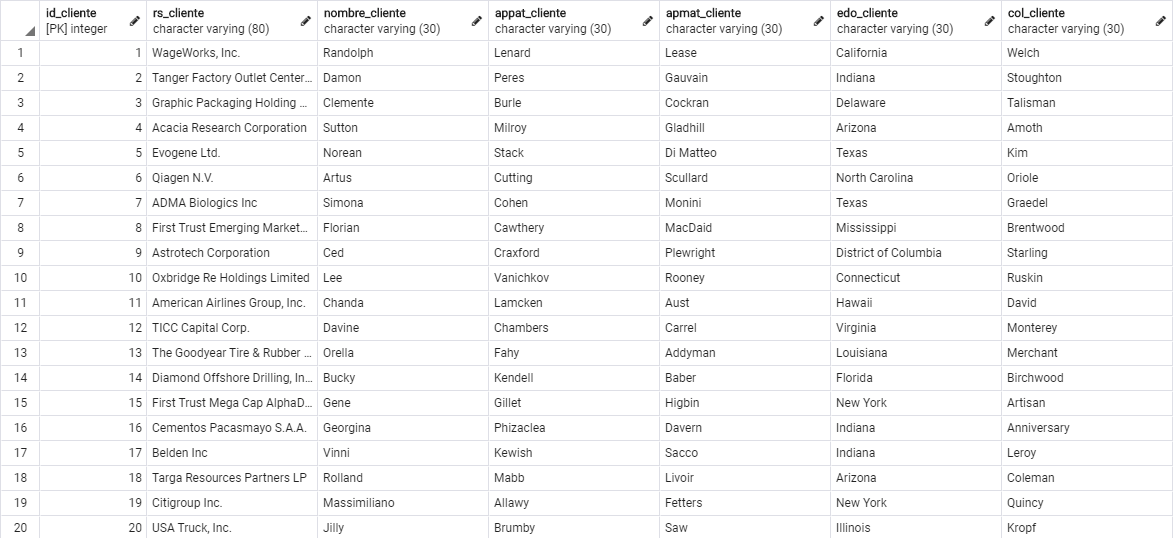
\includegraphics[width=0.95\textwidth]{clienteT.png}
    \caption{Tabla Cliente}
    \label{fig:Tabla Cliente}
\end{figure}

\vspace{15mm} %5mm vertical spac


\textbf{PROVEEDOR:}Se desea almacenar información de aquel que provee productos. 

\vspace{5mm} %5mm vertical space

\begin{figure}[h]
    \centering
    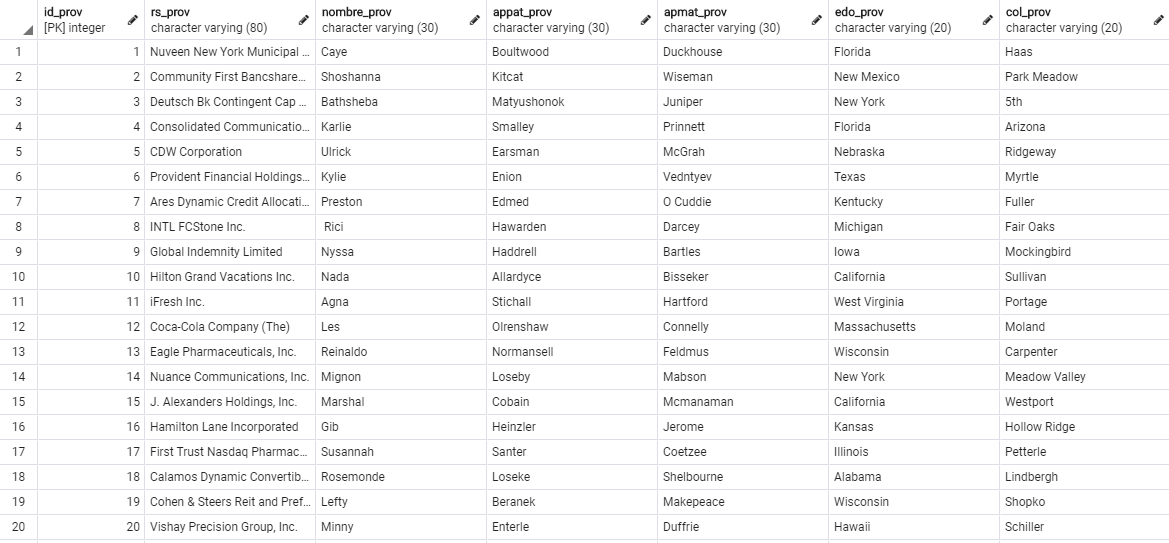
\includegraphics[width=0.95\textwidth]{proveedor.png}
    \caption{Tabla Proveedor}
    \label{fig:Tabla Proveedor}
\end{figure}

\vspace{15mm} %5mm vertical space

\textbf{PRODUCTO:}Se desea almacenar información del producto para venderlo al cliente y tener un registro en el inventario.

\vspace{5mm} %5mm vertical space

\begin{figure}[h]
    \centering
    
\includegraphics[width=0.65\textwidth]{producto.png}
    \caption{Tabla Producto}
    \label{fig:Tabla Producto}
\end{figure}

\vspace{15mm} %5mm vertical space

\textbf{CATEGORÍA:} Se desea dividir en distintas categorías los respectivos productos

\vspace{5mm} %5mm vertical space

\begin{figure}[h]
    \centering
    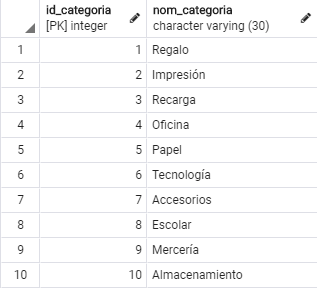
\includegraphics[width=0.35\textwidth]{categoria.png}
    \caption{Tabla Categoria}
    \label{fig:Tabla Categoria}
\end{figure}

\vspace{15mm} %5mm vertical space


\textbf{INVENTARIO:} Se desea almacenar información de los productos que nos permitan relacionarlos con las ventas, dado que tenemos que un precio de compra al proveedor y un precio de venta al cliente, esto con la finalidad de obtener la utilidad.

\vspace{5mm} %5mm vertical space

\begin{figure}[h]
    \centering
    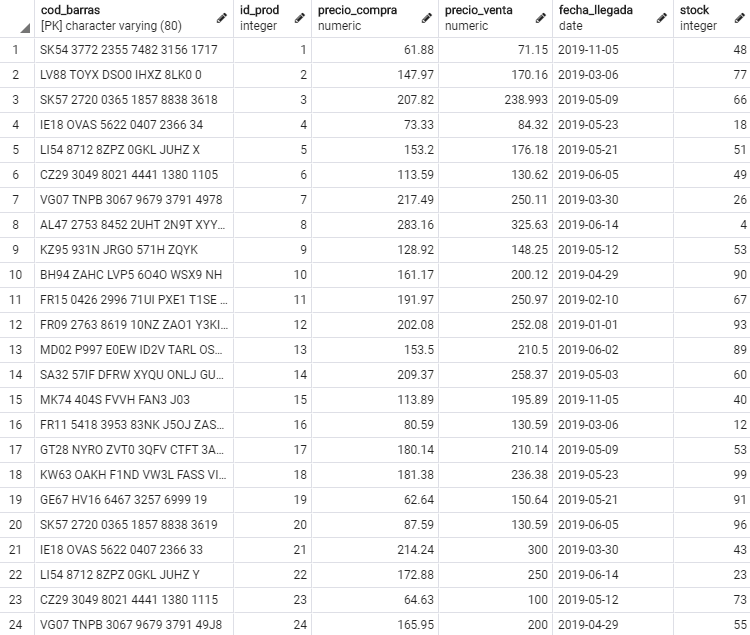
\includegraphics[width=0.55\textwidth]{Inventario.png}
    \caption{Tabla Inventario}
    \label{fig:Tabla Inventario}
\end{figure}

\vspace{15mm} %5mm vertical space


\textbf{VENTA: }Se desea almacenar información de las ventas, de manera que se permita gestionar la salida de los productos, en relación al cliente.

\vspace{5mm} %5mm vertical space

\begin{figure}[h]
    \centering
    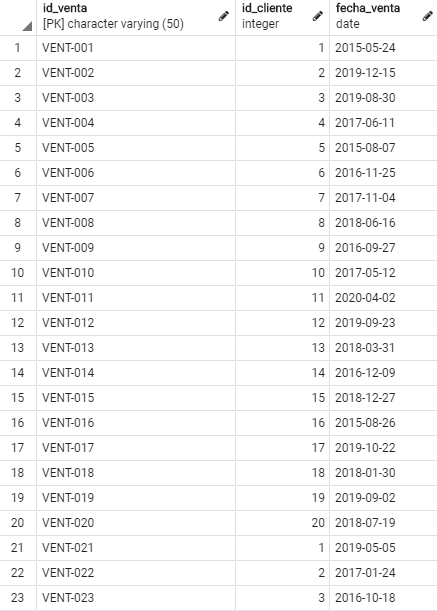
\includegraphics[width=0.30\textwidth]{venta.png}
    \caption{Tabla Venta}
    \label{fig:Tabla Venta}
\end{figure}

\vspace{15mm} %5mm vertical space



\textbf{REGISTRAR:} Se desea almacenar información de las ventas, de manera que se permita gestionar la salida de los productos, en relación al inventario.

\vspace{5mm} %5mm vertical space

\begin{figure}[h]
    \centering
    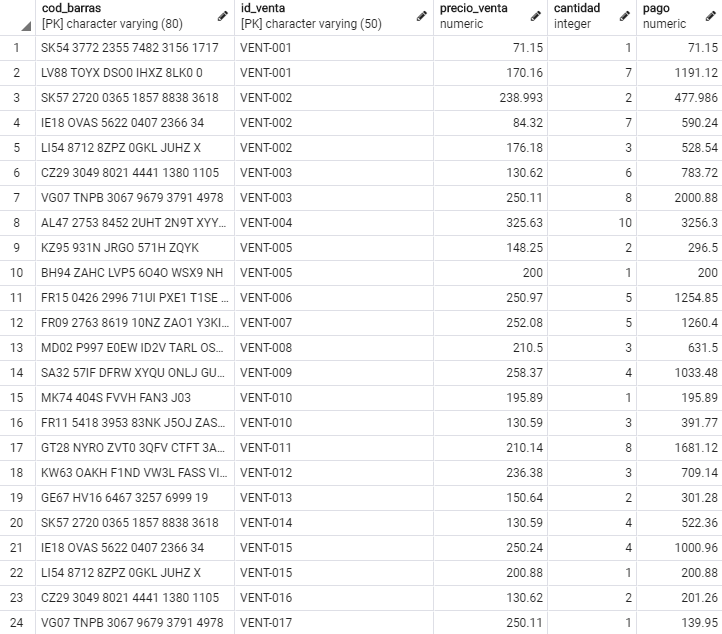
\includegraphics[width=0.75\textwidth]{registrar.png}
    \caption{Tabla Registrar}
    \label{fig:Tabla Registrar}
\end{figure}

\vspace{15mm} %5mm vertical space



%-----------------------------------------------------------------------------------------------------------------------------------------------------------------------------------------------------
\newpage
\subsection{Consultas}\index{Consultas}

\lstset{
    frame=tb, % draw a frame at the top and bottom of the code block
    tabsize=4, % tab space width
    showstringspaces=false, % don't mark spaces in strings
    numbers=left, % display line numbers on the left
    commentstyle=\color{AzulClaro}, % comment color
    keywordstyle=\color{blue}, % keyword color
    stringstyle=\color{gray} % string color
}


\begin{lstlisting}[language=sql, caption={Consulta periodo fecha por producto}]
/*Dada una fecha de inicio y fin, numero de productos vendidos, 
del más vendido al menos. Organizados por producto.*/

CREATE OR REPLACE FUNCTION venta_periodo(varchar, varchar) 
returns TABLE (cod_Barras varchar(80), cantidad bigint)
as
$$
   declare fin date;
   declare inicio date;
   BEGIN 
   fin = date($2);
   inicio = date($1);
   raise notice 'Fecha inicio: %', inicio;
   raise notice 'Fecha fin: %', fin;
   RETURN QUERY SELECT r.cod_barras, sum(r.cantidad)
                       FROM registrar r 
					   inner join VENTA V ON R.id_Venta = V.id_Venta
					   GROUP BY R.COD_BARRAS, R.CANTIDAD, V.ID_VENTA
					   HAVING fecha_Venta>= inicio and fecha_Venta<=fin
					   ORDER BY R.cantidad DESC;		   
   END;
   $$
   LANGUAGE PLPGSQL;
		
--------------REALIZANDO LA CONSULTA --------------------------------

SELECT VENTA_PERIODO('2015-05-24', '2018-05-24');

\end{lstlisting}

\vspace{5mm} %5mm vertical space

\begin{figure}[h]
    \centering
    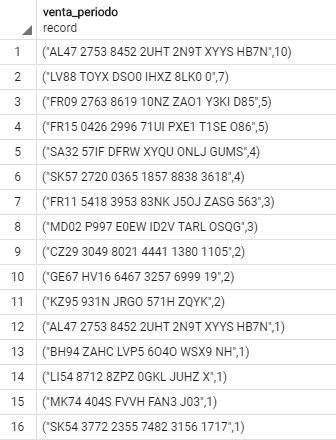
\includegraphics[width=0.35\textwidth]{consultaFecha1.png}
    \caption{Ventas por producto,dado un periodo de fecha}
    \label{fig:Ventas por producto,dado un periodo de fecha}
\end{figure}

\vspace{15mm} %5mm vertical space


\begin{lstlisting}[language=sql, caption={Consulta periodo fecha de productos totales vendidos}]
/*Venta periodo, dada una fecha de inicio y fin, total productos*/

CREATE OR REPLACE FUNCTION TOTALventa_periodo(varchar, varchar) 
 returns int
as
$$
   declare fin date;
   declare inicio date;
   declare totalProductos int;
   BEGIN 
   fin = date($2);
   inicio = date($1);   
   raise notice 'Fecha inicio: %', inicio;
   raise notice 'Fecha fin: %', fin;   
  totalProductos:= (SELECT SUM(R.cantidad) as CantidadProductosVendidos
				FROM Venta V
				INNER JOIN Registrar R ON R.id_Venta=v.id_Venta
				WHERE fecha_Venta between inicio and fin);		   
   	RETURN totalProductos;
   	END;
	$$
	LANGUAGE PLPGSQL;
	
--------------REALIZANDO LA CONSULTA-----------------------------
SELECT totalVENTA_PERIODO('2015-05-24', '2018-05-24');


\end{lstlisting}

\vspace{5mm} %5mm vertical space

\begin{figure}[h]
    \centering
    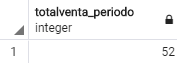
\includegraphics[width=0.35\textwidth]{consultaFecha2.png}
    \caption{Ventas totales,dado un periodo de fecha}
    \label{fig:Ventas totales,dado un periodo de fecha}
\end{figure}

\vspace{15mm} %5mm vertical space




\begin{lstlisting}[language=sql, caption={Función que regresa la utilidad dado un código de barras}]
/*Función que regresa la utilidad dado un código de barras*/
CREATE OR REPLACE FUNCTION UTILIDAD (varchar(80))
RETURNS numeric
AS $$
     declare compra numeric;
	 declare venta numeric;
	 declare utilidad numeric;
    BEGIN
    compra:= (SELECT precio_Compra FROM INVENTARIO i WHERE i.cod_Barras = $1);
    venta := (Select precio_venta FROM INVENTARIO i where i.cod_Barras = $1);
	utilidad = venta - compra;
	RETURN utilidad;
	END;
$$LANGUAGE PLPGSQL;

  
-----------EJECUTANDO LA FUNCION UTILIDAD-----------------------------------
SELECT *FROM utilidad ('GT28 NYRO ZVT0 3QFV CTFT 3AKV RV8Q');


\end{lstlisting}

\vspace{5mm} %5mm vertical space

\begin{figure}[h]
    \centering
    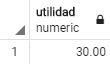
\includegraphics[width=0.25\textwidth]{utilidad.png}
    \caption{Utilidad dado un codigo de barras}
    \label{fig:Tabla Registrar}
\end{figure}


\vspace{5mm} %5mm vertical space


\begin{lstlisting}[language=sql, caption={Factura}]

 /*---------------Vista de una factura-------------------------------*/
CREATE VIEW FACTURA
AS
Select* FROM(
 	SELECT 1 AS Factura, 'Datos de Factura:' as PapeleriaBaseDeDatos, 
	CONCAT('Cliente: ', CAST(C.id_Cliente AS varchar(10))) as Tel55070220,  
	CONCAT('Fecha: ',CAST(V.fecha_Venta AS varchar(10))) as AV20DENOVIEMBRE, 
	CONCAT('Venta: ', v.id_Venta) as Num1024, ' ' as Pago
 	FROM CLIENTE C
	INNER JOIN Venta V ON V.id_Cliente = C.id_Cliente
 	Where v.id_Venta= 'VENT-001'
 UNION
	SELECT 2,CONCAT( 'Facturar A: ',C.appat_Cliente,' ',C.nombre_Cliente), 
	C.rs_Cliente,CONCAT(C.calle_Cliente,' #',C.num_Cliente, ',
	Col.',C.col_Cliente, ', CP.',C.cp_Cliente),
	E.email as CorreoElectronico, ' '
	FROM CLIENTE C
	INNER JOIN Venta V ON V.id_Cliente = C.id_Cliente
 	INNER JOIN email E ON E.id_Cliente = C.id_Cliente
  	Where v.id_Venta= 'VENT-001'
 UNION 
 	SELECT '3', ' ', ' ', ' ', ' ', ' '
 UNION 
 	SELECT '3', 'Codigo Barras', 'Producto', 'Precio unitario', 'Cantidad ', ' '
 UNION
	SELECT 4, r.cod_Barras, P.descripcion as Producto,
	CAST(r.precio_Venta AS varchar(10)), 
	CAST(r.cantidad AS varchar(10)),CAST(r.pago AS varchar(10)) 
	From Venta v
	inner join registrar r on v.id_Venta = r.id_Venta
	inner join inventario I on r.cod_Barras= i.cod_Barras
	inner join producto P on p.id_Prod=i.id_Prod
	Where v.id_Venta= 'VENT-001'
UNION
	SELECT 5, ' ', ' ', ' ', 'SUBTOTAL', CAST(SUM(r.pago) AS varchar(10))
	FROM Venta V
	inner join registrar r on v.id_Venta = r.id_Venta
	Where v.id_Venta= 'VENT-001'
UNION
	SELECT 6, ' ', ' ', ' ', 'IVA 16%', CAST((SUM(r.pago))*0.16 AS varchar(10))
	FROM Venta V
	inner join registrar r on v.id_Venta = r.id_Venta
	Where v.id_Venta= 'VENT-001'
UNION
	SELECT 7, ' ', ' ', ' ', 'TOTAL', CAST((SUM(r.pago)+(SUM(r.pago))*0.16) AS 
	varchar(10))
	FROM Venta V
	inner join registrar r on v.id_Venta = r.id_Venta
	Where v.id_Venta= 'VENT-001'
) as FACT
ORDER BY Factura;

-----------EJECUCION DE FACTURA------------------------------------
Select * From FACTURA

\end{lstlisting}

\vspace{5mm} %5mm vertical space

\begin{figure}[h]
    \centering
    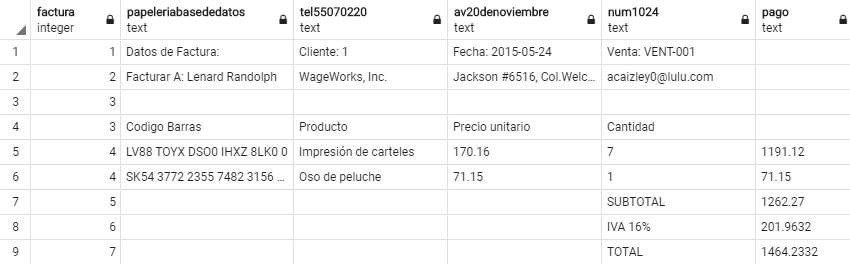
\includegraphics[width=0.75\textwidth]{factura.png}
    \caption{Factura de una venta}
    \label{fig:Factura de una venta}
\end{figure}



\vspace{15mm} %5mm vertical space


\newpage

\begin{lstlisting}[language=sql, caption={Índice}]

/*Creación de índice*/
--El índice se crea en el código de barra, con la finalidad de realizar 
una búsqueda mas rápida al hacer ventas. 

CREATE INDEX Indice_Baras on INVENTARIO(cod_Barras);

\end{lstlisting}

\vspace{15mm} %5mm vertical space

\begin{lstlisting}[language=sql, caption={Verificación de stock}]

/*---------CUANDO STOCK SEA MENOR A 3---------------*/
CREATE OR REPLACE FUNCTION STOCK ()
RETURNS TABLE (cod_Barras varchar(80), cantidad int )
AS 
	$$
	BEGIN 
	RETURN query 
	       SELECT i.cod_Barras, i.stock
		   FROM INVENTARIO i
		   WHERE stock<= 3;
   END;
 $$LANGUAGE PLPGSQL;
 --------------EJECUCION STOCK------------------------  
  select *from stock();

\end{lstlisting}


%----------------------------------------------------------------------------------------
%	PRESENTACIÓN
%-----------------------------------------------------------------------------
\newpage
\section{Presentación}\index{Presentación}

\vspace{5mm} %5mm vertical space

Para la implementación de la interfaz, se identificó el conocimiento de los miembros del equipo acerca de la integración de la base de datos a un entorno gráfico, acorde a los requerimientos del proyecto. Del resultado de ese análisis se decidió desarrollar la interfaz por medio de Java AWT (Abstract Window Toolkit), integrándose con las bibliotecas de Java para manejar bases de datos con SQL.
Posteriormente se determinaron las ventanas y los componentes interactivos necesarios (botones, cuadros de texto, listas, etc.) para que el usuario final intervenga y utilice el sistema de una manera adecuada, asegurando que se respeten las reglas e integridad de la información en la base de datos. Además se asegura que los datos sólo se modifiquen por un determinado usuario con contraseña.  
La interfaz gráfica también fue mejorada en el aspecto estético, colocando el logo y otros elementos gráficos.



\begin{figure}[h]
    \centering
    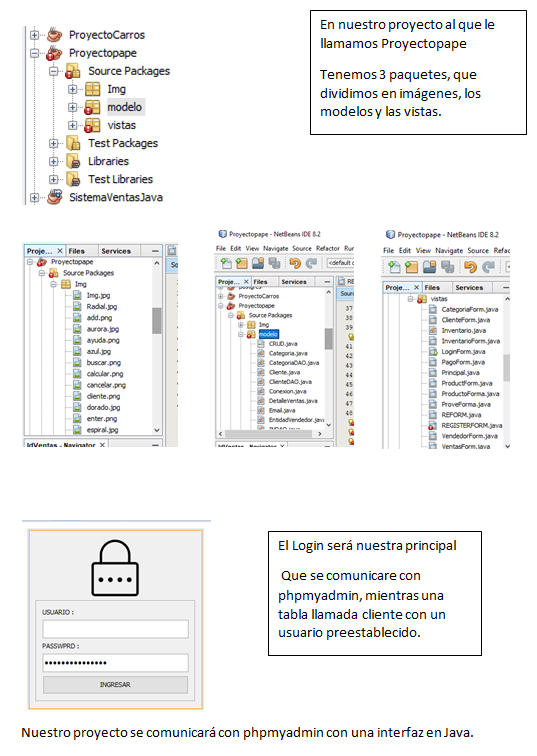
\includegraphics[width=0.65\textwidth]{presentación.png}
    \caption{Interfaz}
    \label{fig:Interfaz}
\end{figure}


%----------------------------------------------------------------------------------------
%	conclusiones
%-----------------------------------------------------------------------------
-------------------

\newpage
\section{Conclusiones}\index{Conclusiones}

Silva Barrera Brandon: 

El proyecto tuvo como dificultad principal, que se reformó al utilizar los avances de dos equipos, por lo que se requirió una buena comunicación y un trabajo de análisis para lograr su integración. Gran parte de los componentes de ambos equipos tuvieron que ser modificados en algunas de sus partes o de forma total, lo que requirió una mayor inversión de tiempo y esfuerzo. El intercambio de ideas entre los nuevos integrantes del proyecto fue fundamental para desarrollar los requerimientos del proyecto con el trabajo ya hecho, por lo que es un acierto tomar en cuenta las opiniones de todos y resolver las diferencias de manera que se llegue a un consenso de cómo se resolverá el proyecto. Las herramientas colaborativas para que todos visualicen el avance del proyecto y lo modifiquen fueron esenciales para el progreso del proyecto, además de tener acceso a información por medio de internet, lo que ayudó a cumplir con el proyecto.

\vspace{10mm} %5mm vertical space

Garcia Cruz Diana Aide:

Para crear bases de datos sólidas es necesario tener los conocimientos de normalización y mapeo así como conceptualizar los requerimientos y el funcionamiento más cercano a la vida cotidiana. Postgres al ser un manejador distinto y diseñado para bases de datos muy grandes nos complicó un poco la parte de programación ya que al no estar familiarizados con su sintaxis y funcionamiento retrasó la entrega del proyecto, por eso mismo se optó por comenzar a utilizar phpMYAdmin ya que para la unión de la aplicación con la base de datos. Poder trabajar en equipo es complejo y el intercambio de ideas lleva a una retroalimentación mutua, en este caso la adaptación de dos proyectos que estaban diseñados para una conceptualización de los datos distinta llevó más tiempo de lo previsto. 

\vspace{10mm} %5mm vertical space

Felix Flores Paul jaime

Creo que aprendimos mucho de este proyecto en cuanto aprendizaje y muchas otras. Aplicamos lo que vimos durante el semestre, incluso aplicamos un poco más con el uso de interfaces en java.
Aprendí más el funcionamiento de todo, así como relacionarlo con Java
Por mi caso decidí aplicar Java, ya que estoy acostumbrado desde Poo hacer proyectos así. Fue muy estresante hacer la base, ya que al ser muchas clases y relaciones entre ellas puff se vuelve complicado. Aprendimos a usar phpMyadmin por el poco tiempo que teníamos como equipo nuevo, postgres era un reto al implementarlo con Java en 4 días. Creo que un poco más de tiempo, me hubiera quedado mejor, pero estoy feliz con mi trabajo.

\vspace{10mm} %5mm vertical space

Jiménez García María Fernanda

El proyecto dio inicio hace algunas semanas, con un diseño similar al propuesto en el presente documento. 
Se realizó la actualización y la mejora de una base de datos de una papelería, con un sistema de ventas.
Durante la elaboración surgieron algunos inconvenientes que se fueron solucionando progresivamente.
El actual sistema está  implementado en java, este mismo, se adecuó a phpmyadmin.
El objetivo era simular una papelería con un sistema que nos permitiera realizar ventas y así,  que permita a los clientes registrarse, seleccionar los productos, comprarlos y pagarlos. 
Sin duda considero las aplicaciones de lo aprendido, como elementales para cualquier tipo de sistema, dado que es necesario guardar permanentemente mucha información.
En este caso particular, algunos de los beneficios serían, tener un control en el manejo de la información, de clientes, del registro de ventas, permitir emitir reportes de ventas, clientes y productos actualizados que, ayudarían a una empresa a tomar mejores decisiones a corto y a largo plazo.
Considero que las condiciones y el tiempo no alcanzaron para que el equipo pudiera conectar ambos trabajos de manera eficiente. 
Por otra parte, SQL es un lenguaje de consulta para los sistemas de bases de datos relacionales, que no posee la potencia de los lenguajes de programación. Por ende, la familiarización con la sintaxis nos fue un poco complicada, y algunas funciones no se implementaron.
Aún con esto, reitero que se aplicaron diversos conocimientos adquiridos a lo largo de la materia  y por lo tanto, se reforzaron.


\vfill
\end{document}